% COLM 2026 submission
\documentclass{article}
\usepackage{colm2026_conference}
\usepackage{graphicx}
\usepackage{booktabs}
\usepackage{amsmath}
\usepackage{hyperref}
\usepackage{xcolor}

\title{Demographic Inference from LLM Residual Streams\\Scales Log-Linearly Across Model Families}

\author{
Anonymous
}

\begin{document}
\maketitle

\begin{abstract}
We probe the residual streams of 22 language models spanning 5 architecture families (Pythia, Gemma~3, Llama~3, Qwen~2.5, Qwen~3) and 3 orders of magnitude in parameter count (14M--14B) to predict author demographics from blog text. Using incremental ridge regression on per-token activations---which requires no activation caching and produces a closed-form solution from a single forward pass---we find that probe accuracy scales log-linearly with model size: $+8.3\%$ per decade on age ($R^2\!=\!0.97$, $p\!<\!10^{-16}$) and $+4.2\%$ per decade on gender ($R^2\!=\!0.92$, $p\!<\!10^{-11}$), with consistent slopes across all families. Zodiac sign prediction remains at chance regardless of scale, confirming the method does not detect spurious correlations. A bag-of-words baseline achieves 65\% on age, while the best 14B probe reaches 76\%, attributing an 11-point gain to contextual processing beyond surface vocabulary. The scaling law, methodology, and trained probes are released for reproducibility.
\end{abstract}

\section{Introduction}

Large language models encode rich representations of their input text in their residual streams. A growing body of probing literature asks what information is linearly decodable from these representations \citep{alain2017understanding, belinkov2022probing, hewitt2019structural}. We focus on a practical question with privacy implications: \emph{can demographic attributes of an author be inferred from a model's internal activations, and how does this capability scale with model size?}

We make three contributions:
\begin{enumerate}
    \item \textbf{A scaling law for demographic probing.} Across 22 models from 5 families spanning 3 orders of magnitude (14M--14B parameters), ridge probe accuracy scales log-linearly with parameter count, with a consistent slope across architectures (Figure~\ref{fig:scaling}).
    \item \textbf{Incremental ridge probing methodology.} We accumulate the Gram matrix $X^\top X$ and cross-covariance $X^\top Y$ during a single forward pass, then solve in closed form. This eliminates the need for activation caching, avoids SGD convergence issues, and produces results invariant to batch size.
    \item \textbf{Signal decomposition.} We decompose probe accuracy into vocabulary signal (bag-of-words baseline), embedding signal (layer~0 probe), and contextual signal (best layer minus layer~0), showing that larger models contribute primarily through contextual processing.
\end{enumerate}

\section{Method}

\subsection{Data}

We use the Blog Authorship Corpus \citep{schler2006effects}, comprising blog posts with author metadata. We predict three attributes: age bin (13--17, 23--27, 33--47; 3-class), gender (2-class), and zodiac sign (12-class, as a negative control). Posts are filtered to $\geq\!50$ tokens, balanced by age bin at the blogger level, and split 70/15/15 by blogger to prevent leakage.

\subsection{Probing}

For each model, we run a single forward pass over 100K training texts with hooks capturing the residual stream at every 4th layer. For each non-padding token at each hooked layer, we extract the activation vector $\mathbf{h} \in \mathbb{R}^D$ and assign it the text's demographic label.

\paragraph{Incremental Ridge Regression.} Rather than caching activations, we accumulate sufficient statistics on GPU during the forward pass:
\begin{align}
    \mathbf{A} &\mathrel{+}= \mathbf{X}^\top \mathbf{X}, \quad
    \mathbf{B} \mathrel{+}= \mathbf{X}^\top \mathbf{Y}, \quad
    \boldsymbol{\mu} \mathrel{+}= \textstyle\sum \mathbf{x}_i
\end{align}
where $\mathbf{X}$ is the batch of token activations and $\mathbf{Y}$ is the one-hot label matrix. After training, we z-score and solve:
\begin{equation}
    \mathbf{W} = \left(\frac{\mathbf{A}_z}{n} + \lambda \mathbf{I}\right)^{-1} \frac{\mathbf{B}_z}{n}
\end{equation}
with $\lambda$ selected on a validation set. This requires $O(D^2)$ memory per layer (64MB for $D\!=\!4096$) versus terabytes for full activation caching, and produces identical results to offline ridge regression.

\paragraph{Evaluation.} At test time, the probe predicts per-token, and logits are averaged across all tokens in a text before taking the argmax. We report balanced accuracy (macro-averaged recall).

\paragraph{Additional probes.} We also train online EMA linear probes (7 hyperparameter configurations), MLP probes (hidden sizes 16--128), attention probes \citep{dower2024attention}, and a shuffled-label control, all sharing the same forward pass.

\subsection{Models}

We probe 22 base (pretrained) models across 5 families: Pythia 14M--1B \citep{biderman2023pythia}, Gemma~3 270M--12B, Llama~3 1B--8B, Qwen~2.5 0.5B--14B, and Qwen~3 0.6B--8B. All are loaded in bfloat16.

\section{Results}

\subsection{Scaling Law}

\begin{figure}[t]
    \centering
    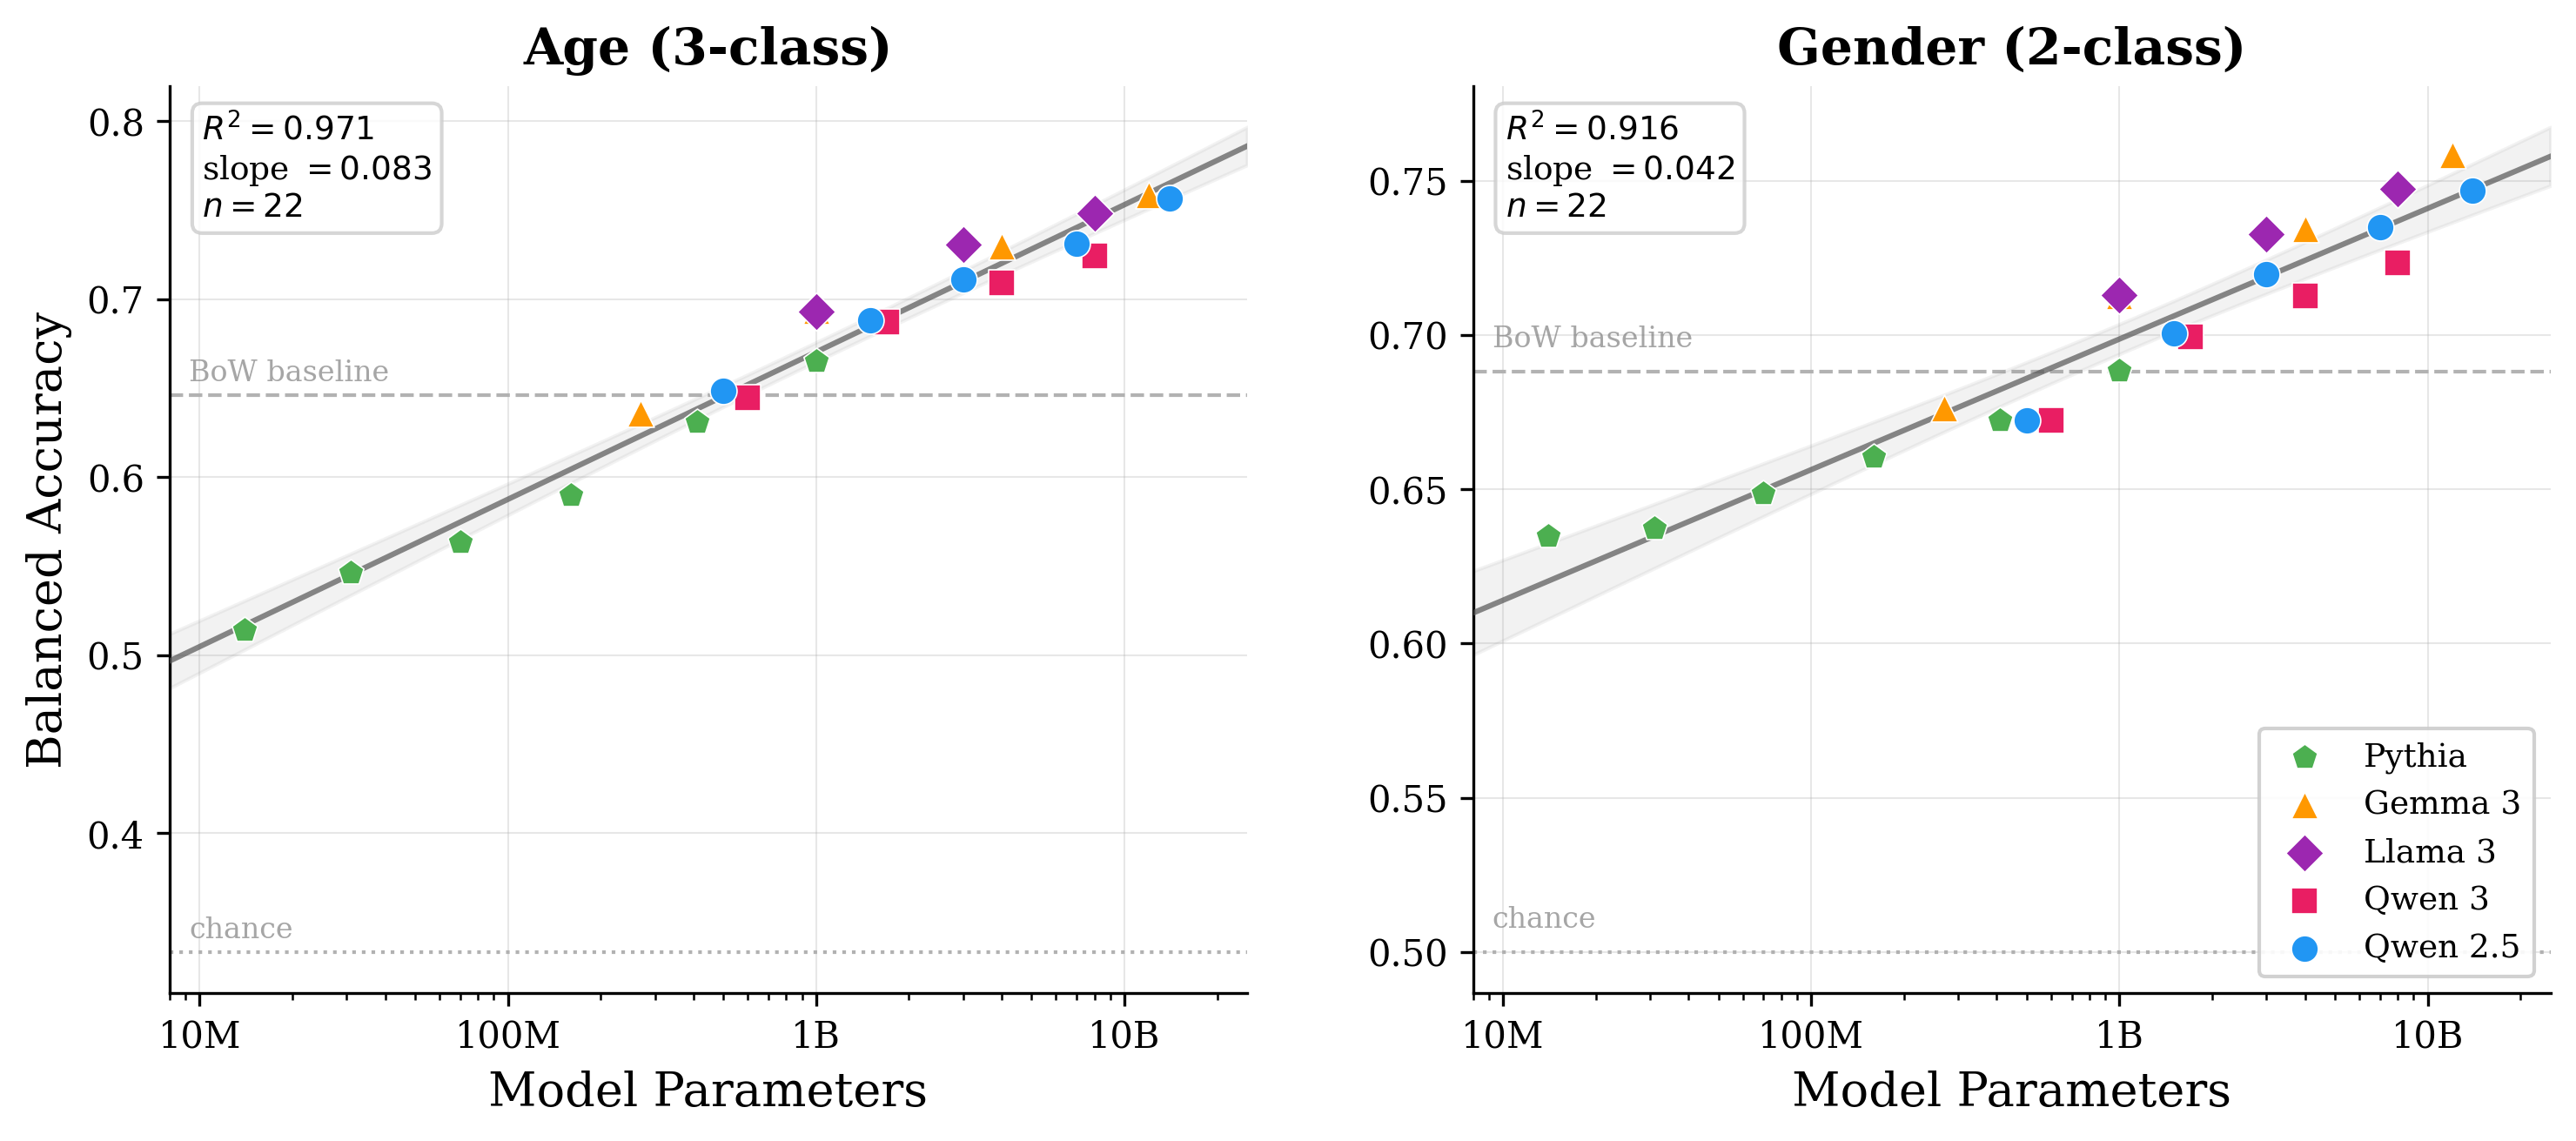
\includegraphics[width=\linewidth]{figures/paper_scaling_law.png}
    \caption{Ridge probe accuracy vs.\ model parameters (log scale) for age and gender prediction. Each point is one model's best-layer accuracy. The dashed line is a log-linear fit across all 22 models ($R^2\!=\!0.97$ for age, $0.92$ for gender). The BoW baseline (TF-IDF + logistic regression on raw text) is shown for reference. Zodiac sign (not shown) remains at chance ($8.3\%$) for all models.}
    \label{fig:scaling}
\end{figure}

Probe accuracy scales log-linearly with parameter count (Figure~\ref{fig:scaling}). For ridge regression on age: $\text{acc} = 0.083 \cdot \log_{10}(N) + 0.69$ with $R^2\!=\!0.97$ ($p\!<\!10^{-16}$, $n\!=\!22$). For gender: slope $= 0.042$, $R^2\!=\!0.92$ ($p\!<\!10^{-11}$). All five model families follow the same slope; a family-intercept model achieves $R^2\!=\!0.985$ on age, with Llama and Gemma ~2\% above the Qwen baseline.

Zodiac sign accuracy hovers at chance ($8.3\%$) across all models and all probe types, confirming that the method does not detect spurious high-dimensional correlations.

\subsection{Signal Decomposition}

\begin{figure}[t]
    \centering
    
\includegraphics[width=\linewidth]{figures/paper_signal_decomposition.png}
    \caption{Decomposition of probe accuracy into embedding-layer signal (layer~0, blue) and contextual gain (best layer minus layer~0, green). The BoW baseline (orange dashed) provides the vocabulary-only reference. Contextual gain grows with model size.}
    \label{fig:decomp}
\end{figure}

A bag-of-words baseline (TF-IDF + logistic regression) achieves 65\% on age and 69\% on gender using vocabulary alone. Ridge probes at layer~0 (embeddings, no context) achieve $\sim$42\% on age and $\sim$59\% on gender---below the BoW baseline, since the embedding compresses 50K+ vocabulary into $D$ dimensions.

The contextual gain (best layer minus layer~0) scales with model size: from $+23\%$ at 0.5B to $+34\%$ at 14B for age (Figure~\ref{fig:decomp}). This gain represents what the transformer's contextual processing adds beyond surface vocabulary.

\subsection{Layer Profile}

\begin{figure}[t]
    \centering
    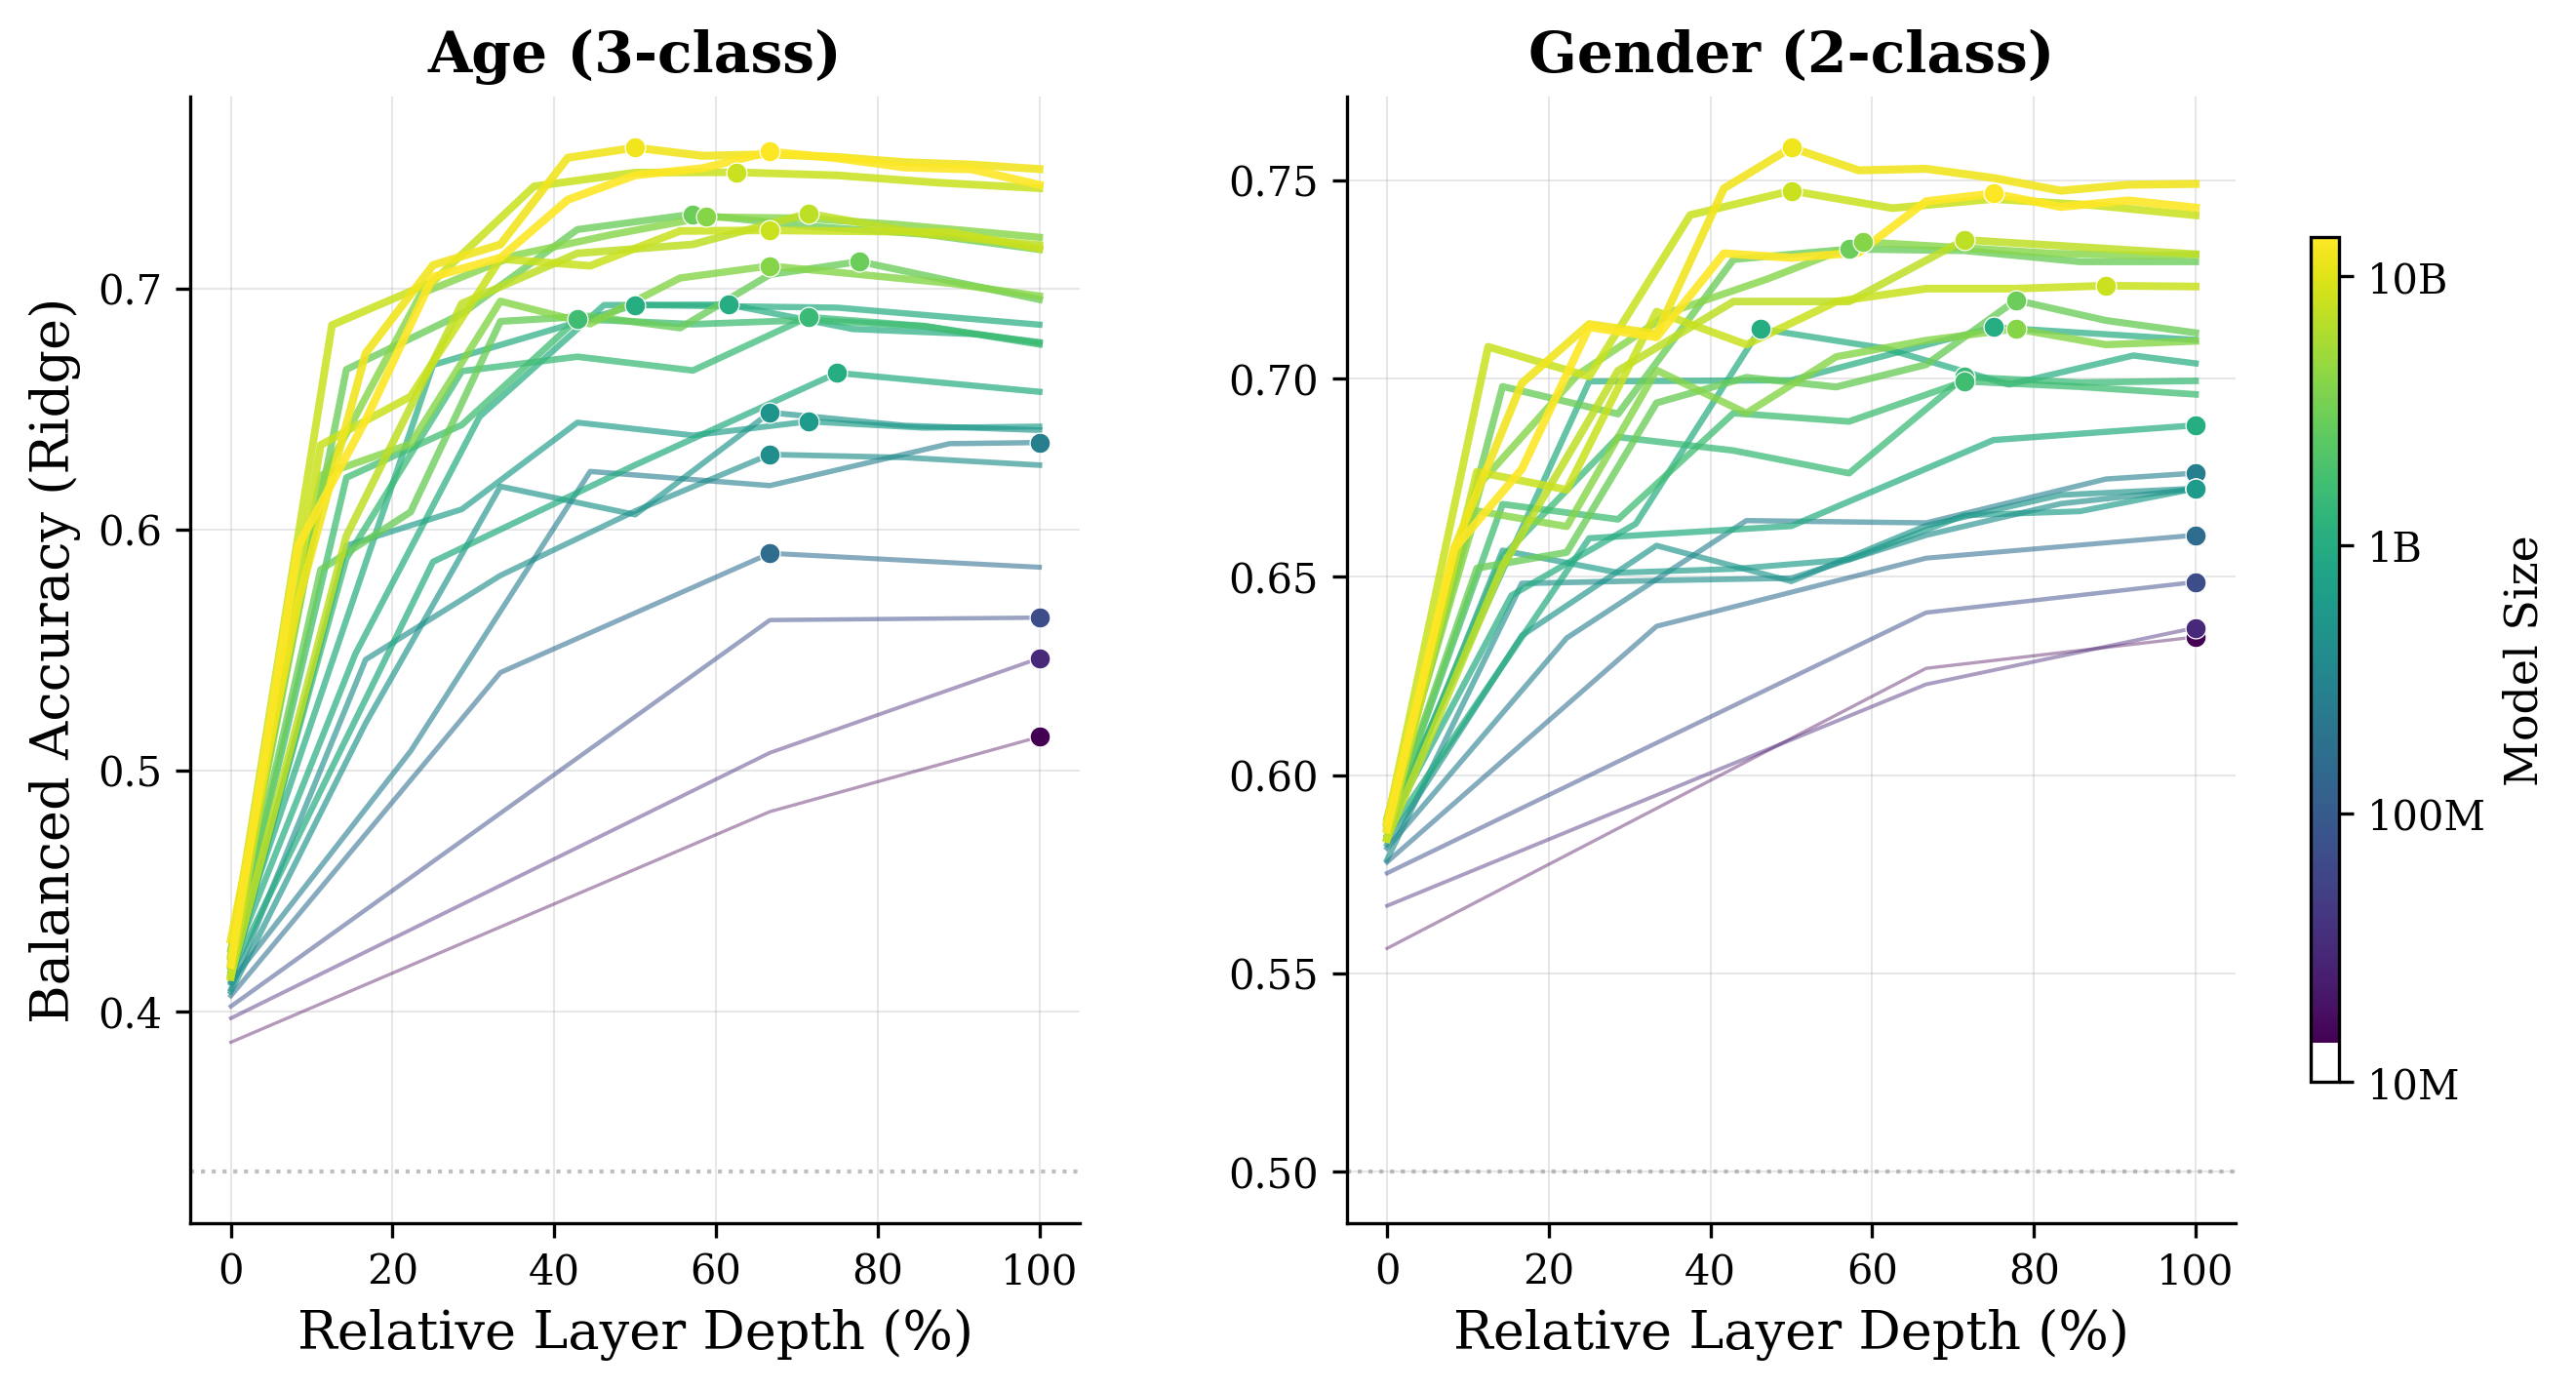
\includegraphics[width=\linewidth]{figures/paper_layer_all_models.png}
    \caption{Ridge accuracy by relative layer depth for all 22 models. Accuracy peaks at 60--75\% depth, not at the final layer. Color indicates model size (log scale).}
    \label{fig:layers}
\end{figure}

Demographic signal builds through the first $\sim$70\% of the network and plateaus or slightly declines in the final layers (Figure~\ref{fig:layers}). This is consistent across all families and suggests that the final layers, which are optimized for next-token prediction, may discard some demographic information.

\subsection{Probe Architecture Comparison}

MLP probes outperform linear probes at small scale (e.g., +7\% at 0.5B) but converge at larger scale ($<$1\% gap at 7B+), suggesting that demographic information becomes more linearly encoded in larger models. The attention probe is competitive but unstable across layers due to its small parameter count. All probe types agree on the scaling trend.

\section{Discussion}

\paragraph{Limitations.} The primary confound is that demographic groups use different vocabulary and topics. The BoW baseline quantifies this: 65\% of the age signal is accessible from word frequencies alone. The remaining 11 points (at 14B) represent the LLM's contextual contribution, but we cannot fully rule out that this reflects stylistic patterns rather than genuine demographic representations. Cross-domain transfer or lexical neutralization experiments would help disentangle these.

\paragraph{Privacy implications.} Even a 14M-parameter model extracts above-chance demographic signal from arbitrary text. This scales predictably with model size, suggesting that larger deployed models encode substantially more author information in their residual streams.

\paragraph{Methodological contribution.} Incremental Gram matrix probing eliminates the standard probing pipeline's reliance on cached activations. The sufficient statistics ($\mathbf{X}^\top \mathbf{X}$, $\mathbf{X}^\top \mathbf{Y}$) can be accumulated during a single inference pass and solved offline for arbitrary regularization strengths.

\section{Conclusion}

Demographic probe accuracy scales log-linearly with model parameters across 5 architecture families and 3 orders of magnitude, with a universal slope of $+8.3\%$/decade for age and $+4.2\%$/decade for gender. This scaling law holds from 14M to 14B parameters with $R^2 > 0.92$. We release all probes, Gram matrices, and code for reproducibility.

\bibliography{main}
\bibliographystyle{colm2026_conference}

\end{document}
